%% -*- coding:utf-8 -*-
\section{Упражнения}
\begin{enumerate}
\item Исходя из (\ref{eqCh2_task21}), получить выражение
  (\ref{eqCh2_task22}) для оператора $\hat{V}$ в представлении
  взаимодействия. 
\item Вывести систему уравнений (\ref{eqCh2_task3}).
\item Получить формулу (\ref{eqCh2_task4}).
\item Вывести из (\ref{eqCh2_rho_final2}) уравнение для матрицы
  плотности в представлении чисел заполнения (\ref{eqCh2_task5}). 
\item Привести формулу (\ref{eqCh2_66}) к виду (\ref{eqCh2_69}).
\item Интегрируя по частям, получить выражения (\ref{eqCh2_70}),
  (\ref{eqCh2_71}).
\item Записать общее уравнение (\ref{eqCh2_73}) в полярной системе
  координат (\ref{eqCh2_77}). 
\item Записать общее уравнение (\ref{eqCh2_73}) в прямоугольной
  системе координат (\ref{eqCh2_77a}). 
%\item Получить из (\ref{eqCh2_75}) уравнение (\ref{eqCh2_76}).
\item Вывести соотношения (\ref{eqCh2_96}) и (\ref{eqCh2_96_add}).
\item Вывести уравнение (\ref{eqCh2_97}).
\item Доказать (\ref{eqPart1Ch2_Lanzgeven_Task1}) и (\ref{eqPart1Ch2_Lanzgeven_Task2}).
\item Получить выражение (\ref{eqPart1Ch2_Lanzgeven_Task3}).
\item Вы хотите измерить частоту перехода между двумя состояниями
  \begin{figure}
    \centering
    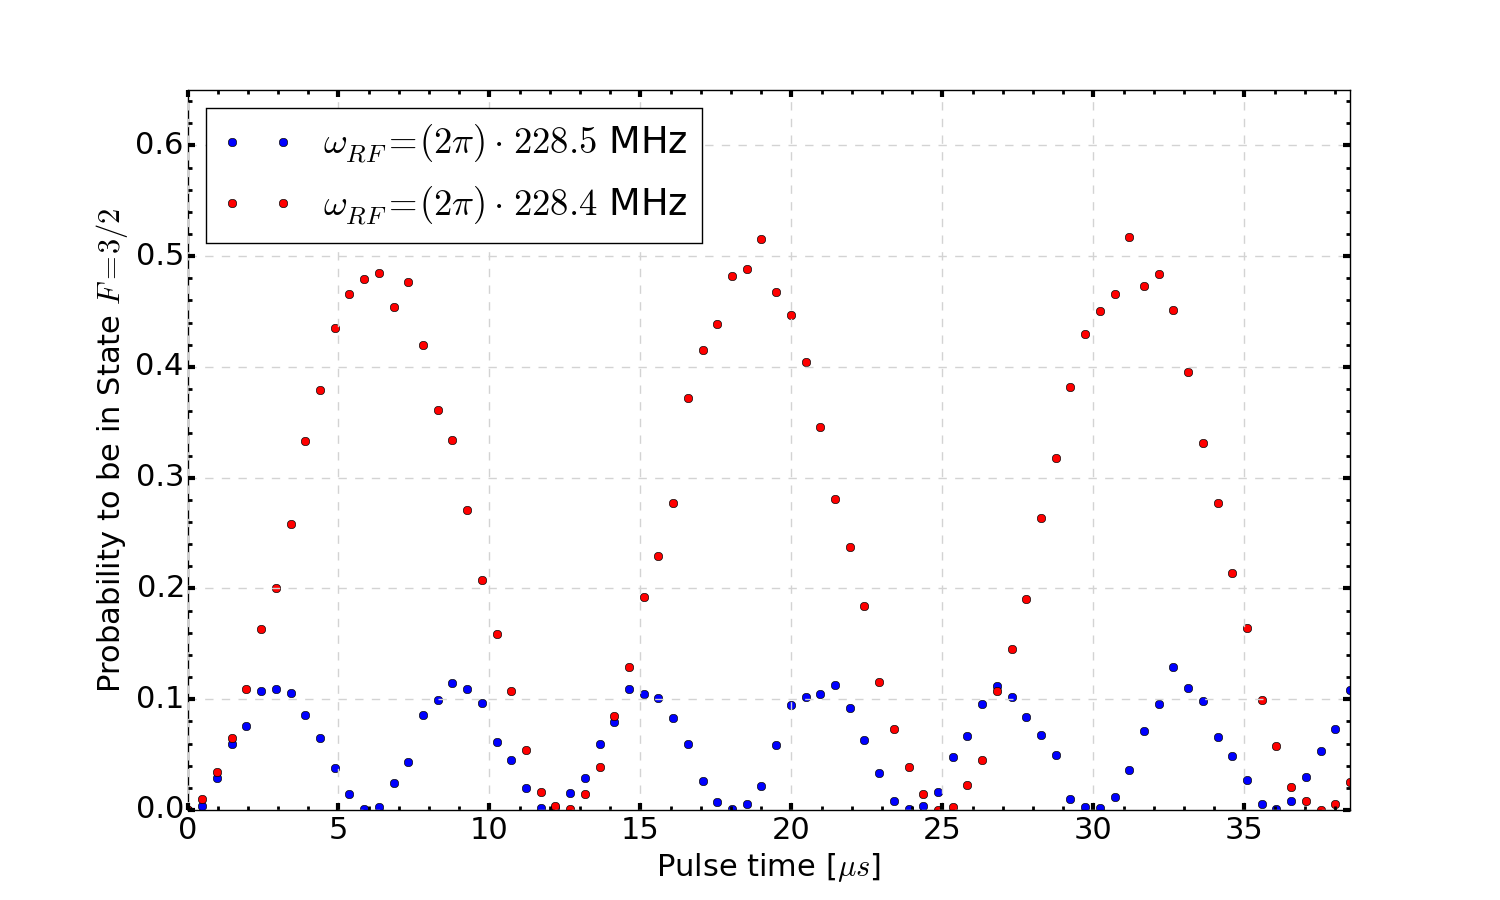
\includegraphics[natwidth=800,natheight=600,width=\textwidth]{part1/interaction/RabiOscillations2_v3.png}
    \caption{Результат эксперимента}
    \end{figure}
\end{enumerate}
